\documentclass{article}

\usepackage{tikz}
\usetikzlibrary{angles, quotes} % ←これが必要!

%picコマンドのマクロ(青い中心と円)
\tikzset{
  mycircle/.pic = {
    \draw[blue, thick] (0,0) circle(5pt);
    \fill[blue] (0,0) circle(1pt);
  }
}

\begin{document}
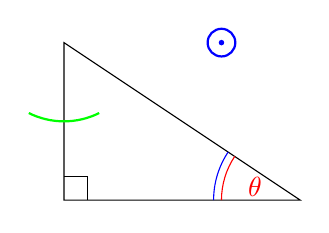
\begin{tikzpicture}
% 三角形の3点
\coordinate (A) at (0,0);
\coordinate (B) at (3,0);
\coordinate (C) at (0,2);

%円弧を描くための座標設定
\coordinate (D1) at (1,0);
\coordinate (D2) at (-1,0);

% 三角形の辺
\draw (A) -- (B) -- (C) -- cycle;

% 直角記号を描く(角BAC)
\path pic[draw, angle radius=0.3cm, angle eccentricity=1.1] {right angle = B--A--C};

%角度の記号、ラベルθ
\path pic["$\theta$", draw, angle radius=1cm,red] {angle = C--B--A};
%さらに外側に角度
\path pic[draw, angle radius=1.1cm,blue] {angle = C--B--A};

%マクロを使用
\path (2,2) pic {mycircle};

%設定したD1とD2を使って、円弧を描く
\path pic[draw, angle radius=1cm,green,thick] {angle = D2--C--D1};
\end{tikzpicture}
\end{document}
